\begin{figure}[!t]
\centering
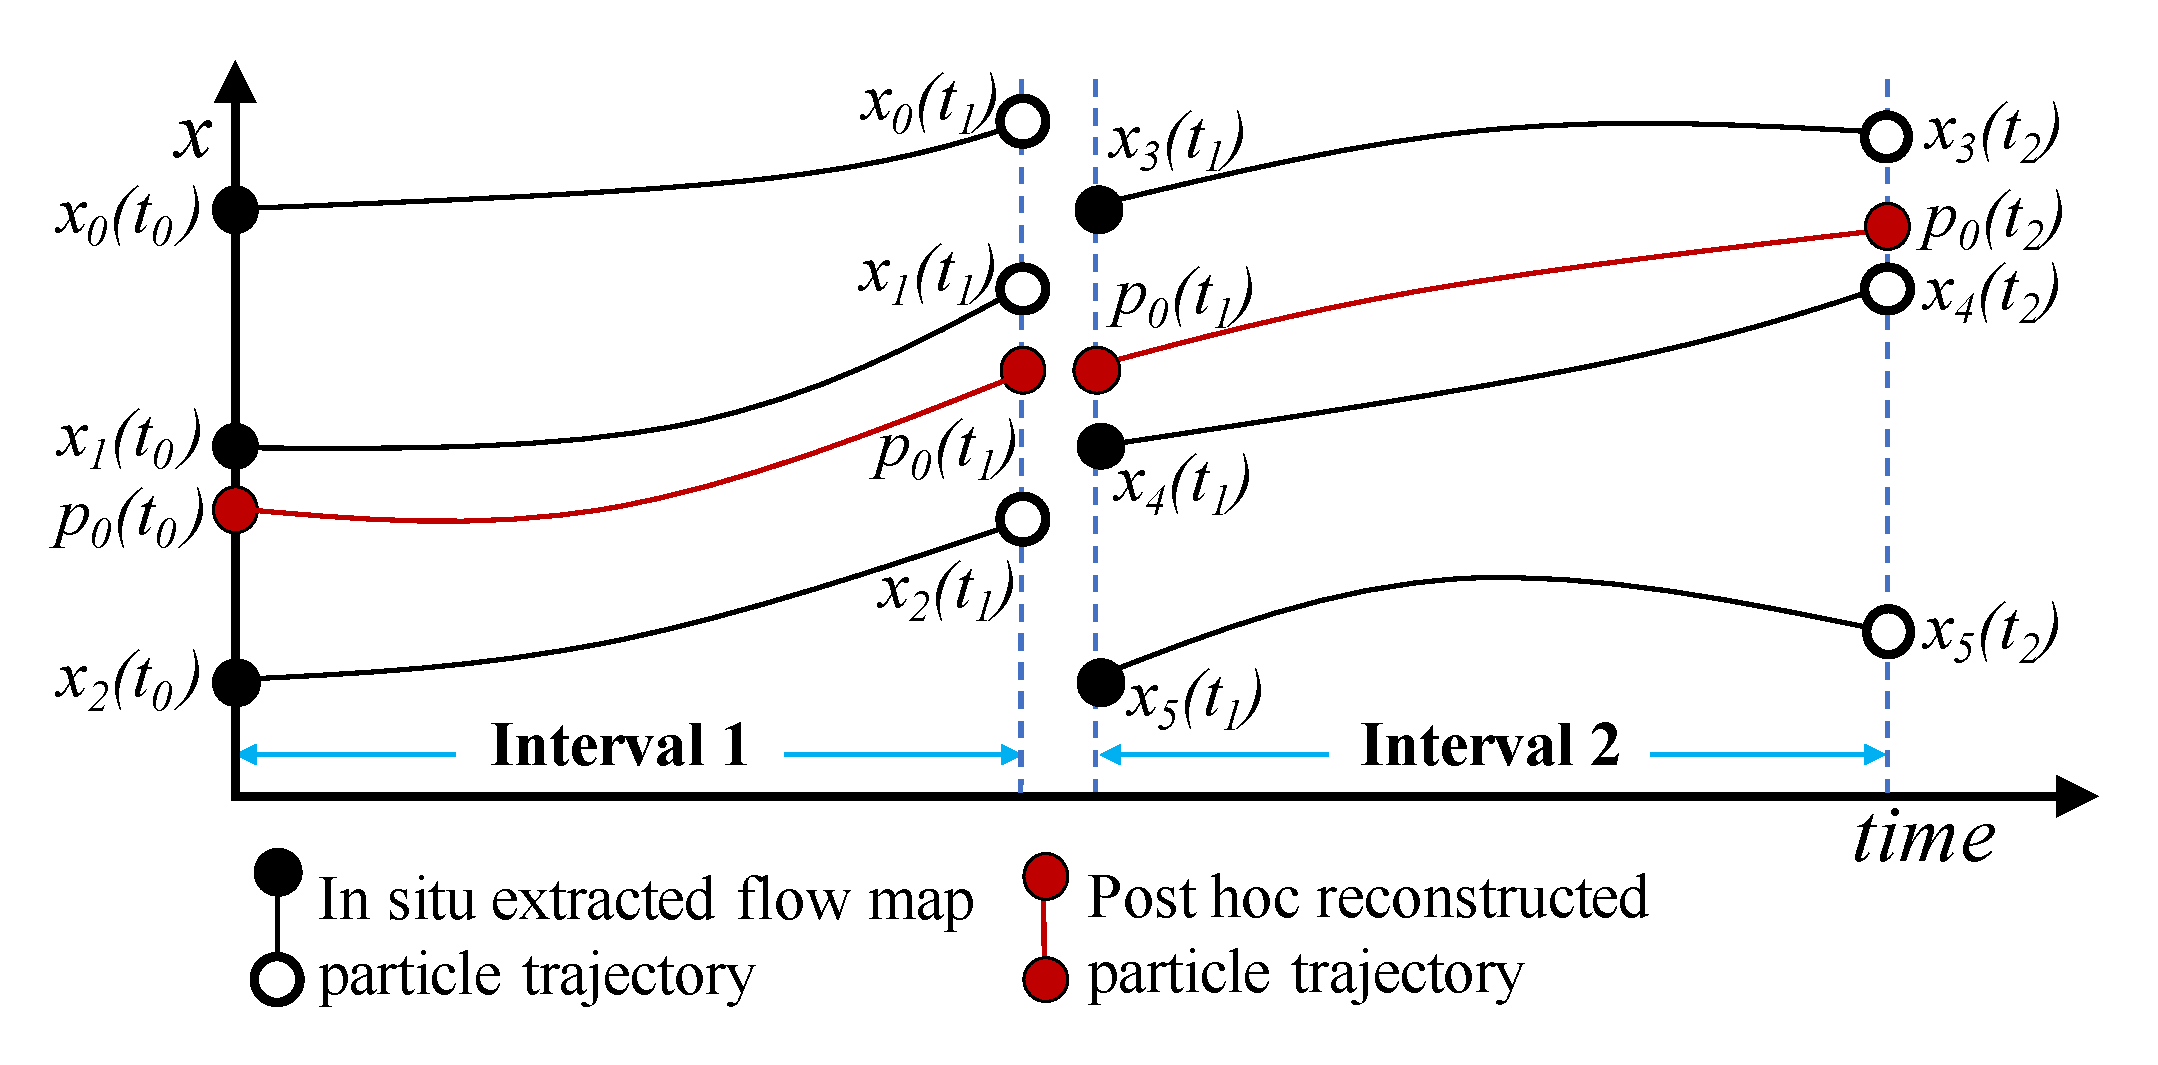
\includegraphics[width=\linewidth]{Images/phases_new_tall.eps}
\caption{The phases of Lagrangian analysis. The in situ phase uses uniform seed placement and extracts flow maps over temporally nonoverlapping intervals. 
%
In this example, the flow maps for the intervals [$t_0$, $t_1$] and [$t_1$, $t_2$] consist of particles \{$x_0$, $x_1$, $x_2$\} and \{$x_3$, $x_4$, $x_5$\}, respectively. 
%
The extracted flow maps are used as input during the post hoc phase. 
%
Here, the trajectory of particle $p_0$ is calculated by interpolating the flow maps, i.e., from $x_1$ and $x_2$ in the first time interval, and $x_3$ and $x_4$ in the second time interval.}
\vspace{-8mm} 
\label{fig:phases}
\end{figure}
